\documentclass[a4paper, oneside, 12pt]{article}

\usepackage[utf8]{inputenc}
\usepackage[T1]{fontenc} 
\usepackage[ngerman]{babel}

\usepackage{parskip}
\usepackage{setspace}
\onehalfspacing

\usepackage[bookmarks, pageanchor, hidelinks]{hyperref}
\usepackage[left=2.5cm, right=4cm, top=2.0cm, bottom=2.0cm]{geometry}

\usepackage{amsmath}
\usepackage{amsfonts}
\usepackage{graphicx}


\title{Detektion von planar aufgenommenen QR-Codes}
\author{Christian Dielitz, Simon Leistikow, Frederik }

\begin{document}
	
\maketitle
\newpage

\tableofcontents
\newpage

\section{Einleitung}
\label{s:einleitung}
In der heutigen, digitalen Welt wird der einfache und schnelle Austausch von Informationen immer wichtiger. Als eines von vielen Kommunikationsträger dient dabei der sogenannte Quick Response (kurz QR) Code, da er Informationen gut komprimieren und durch bestimmte Software schnell wieder zurück verarbeitet werden kann.

Ein QR-Code ist im wesentlichen ein Raster von schwarzen und weißen Flächen, welche Quadratisch angeordnet sind. In aktuelleren Standards ist es allerdings auch erlaubt, kleinere Bilder (wie z.B. Firmenlogos) in den QR-Code zu integrieren. Heutzutage sind QR-Codes sehr populär und werden meist zur Kodierung von Internetseiten verwendet. Der Einsatzbereich eines QR-Codes beschränkt sich allerdings nicht nur auf URL Komprimierung: Mit seiner Hilfe lässt sich jeder beliebige Text, Bilder oder sogar Hologramme kompakt darstellen. Ein wesentliches Problem von QR-Code ist allerdings, das nicht direkt ersichtlich ist, welche Daten ein QR-Code enthält. Beispielsweise wäre es möglich Schadsoftware zu kodieren, welche beim Lesen ausgeführt wird und das entsprechende Lesegerät befällt.

Da die Eingabe eines QR-Codes meist durch ein aufgenommenes Bild einer Kamera vorliegt, ist es unumgänglich, dass eine schnelle Lokalisierung und des QR Codes durchgeführt werden muss.

Innerhalb diese Praktikums haben wir uns damit auseinander gesetzt, wie man planar aufgenommene QR-Codes möglichst schnell und zuverlässig aus einem Bild extrahieren kann. Dazu haben wir, basierend auf OpenCV, ein Programm entwickelt, welches sowohl Bilder von der Webcam eines Computers aufnehmen als auch schon gespeicherte Bilder laden kann und den  darin enthaltenen QR Code als eigenständiges Bild extrahiert.

\newpage
\section{Grundlagen}
\label{s:grundlagen}
\subsection{Aufbau eines QR-Codes}
\label{ss:aufbau}
Ein QR-Code in eine Matrix $M = n \times n$ (auf Grund der aktuellen Standards gilt $n \in \{21,...,177\}$) welche die kodierten Daten in Binär Form darstellt. Ein schwarzes Quadrat stellt dabei eine 1 dar und ein leeres, weißes Feld eine 0. In einem QR-Code lassen sich also maximal bis zu $n*n$ Bits speichern.

\begin{figure}[h]
	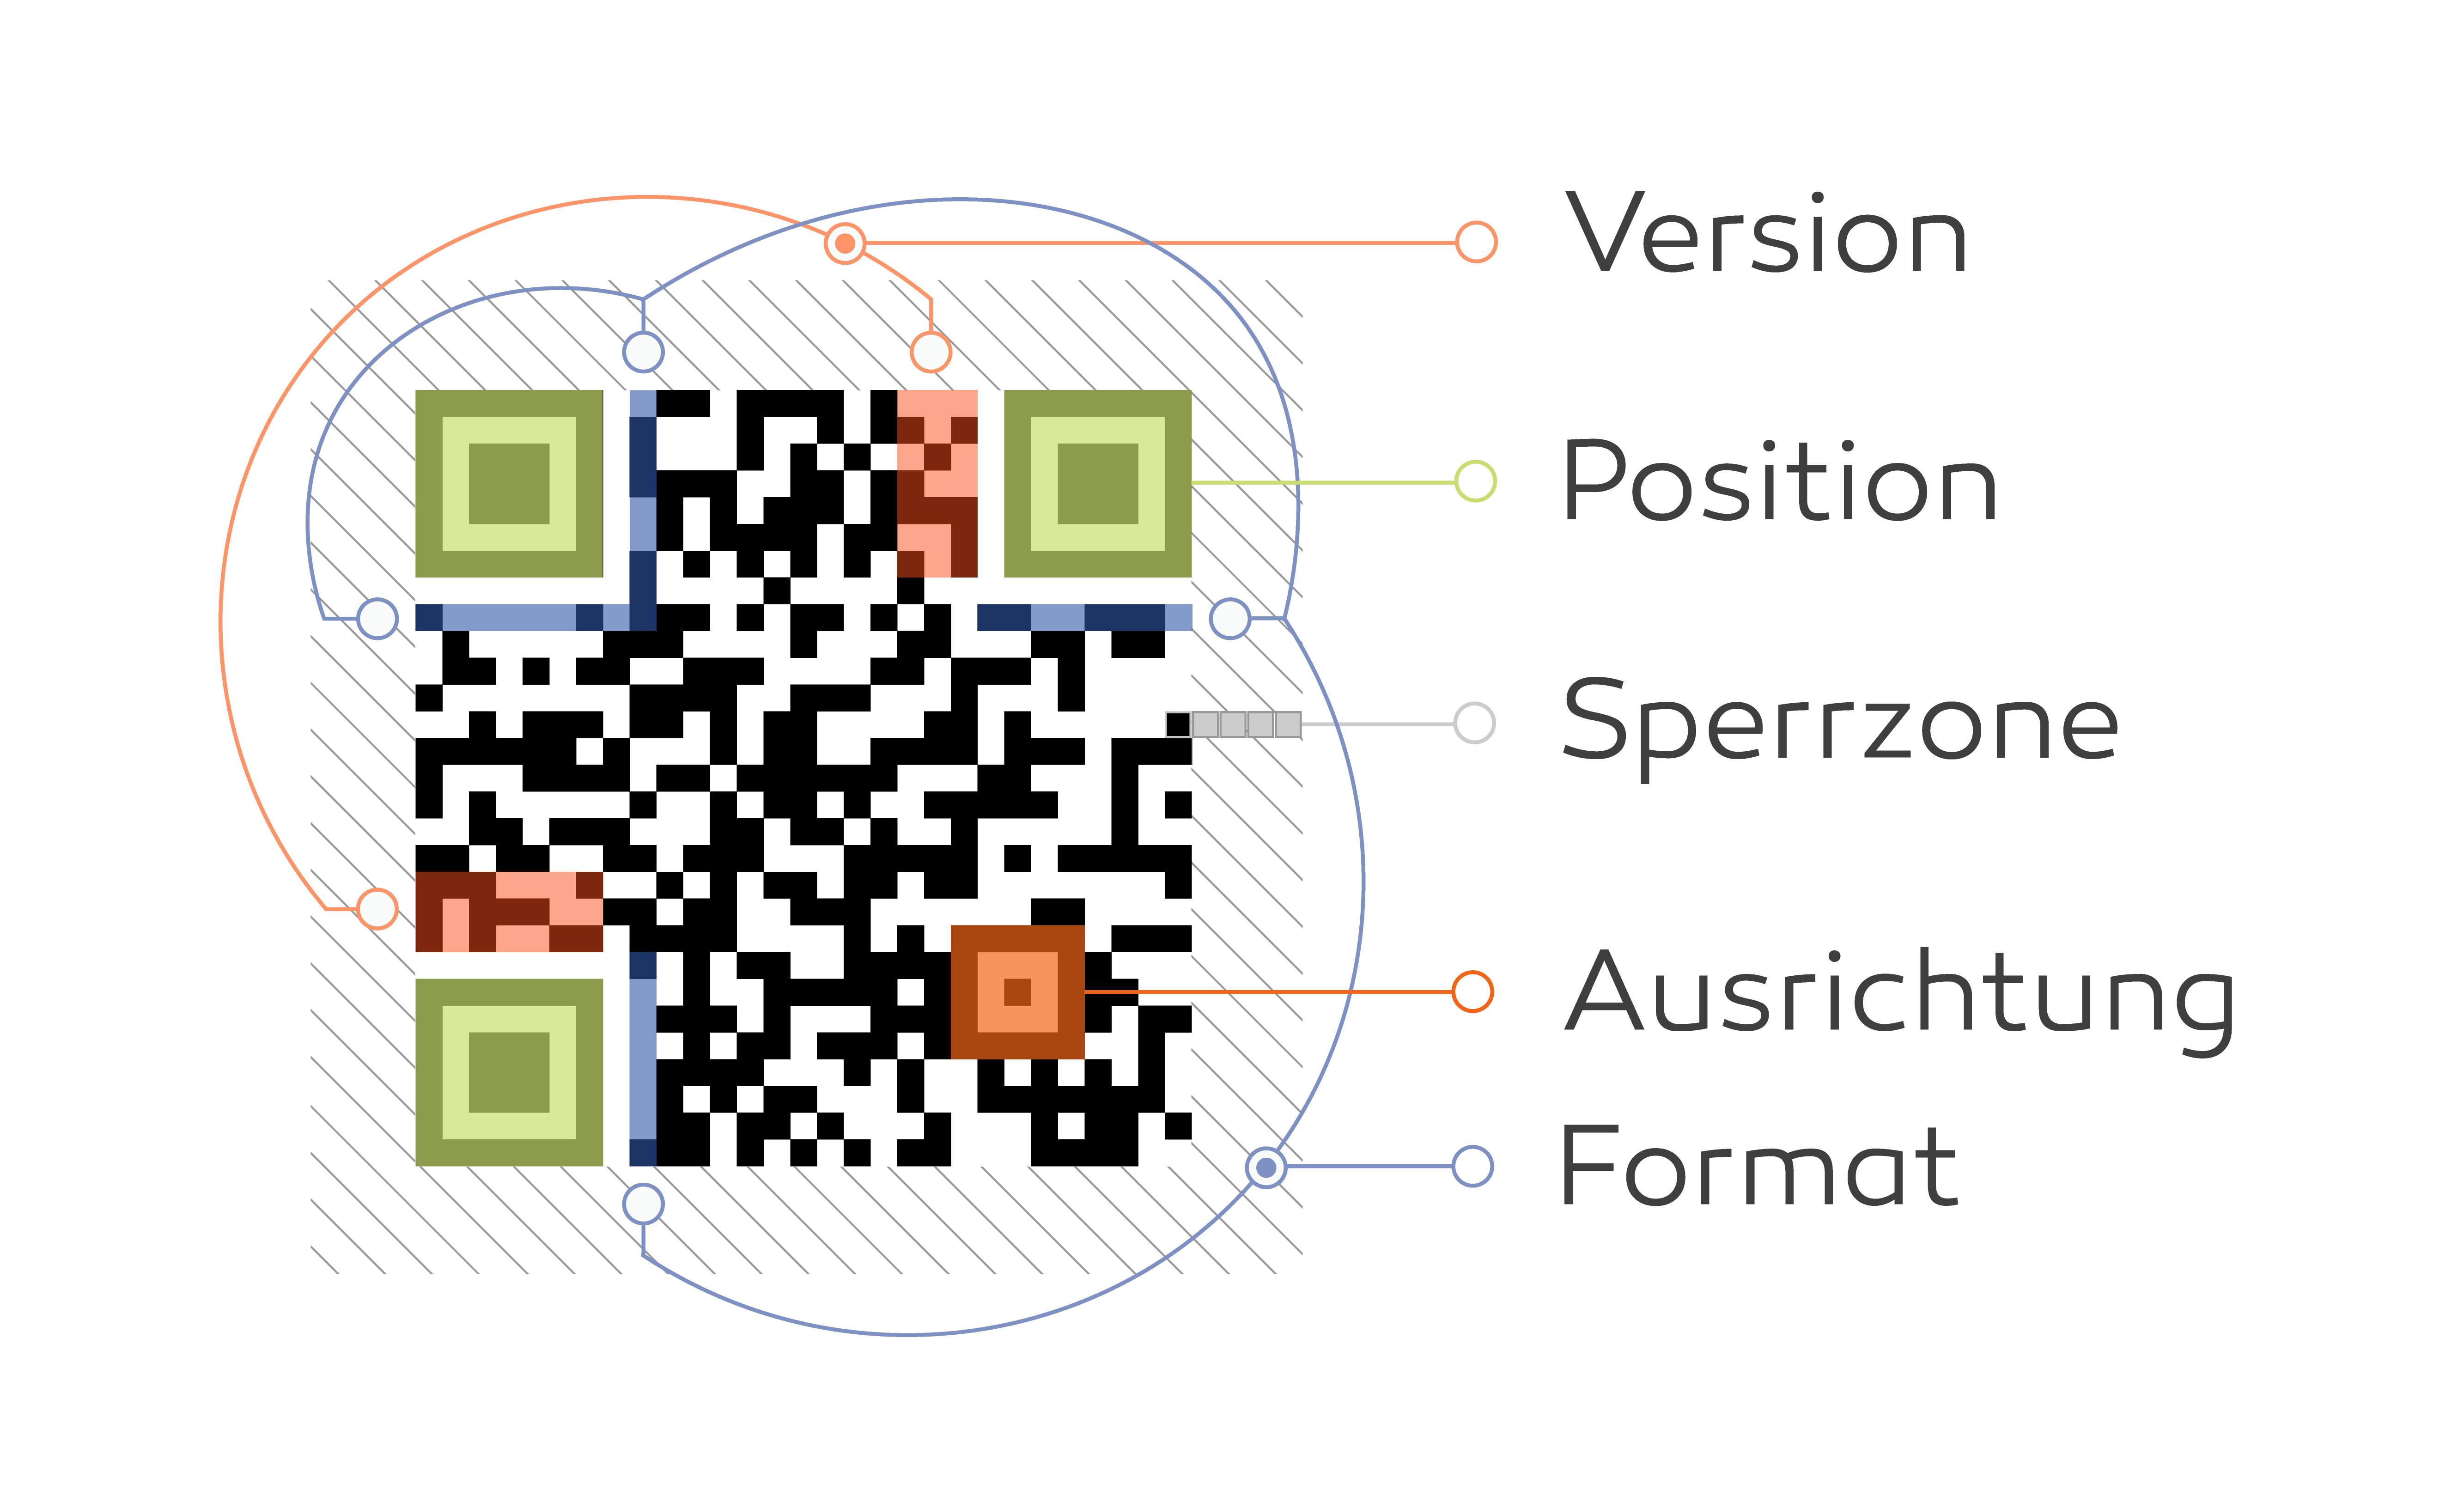
\includegraphics[width=\textwidth]{images/aufbau.png}
	\caption{Aufbau eines Beispiel QR-Codes}
	\label{fig:aufbau}
\end{figure}

Jeder QR-Code ist von einer sogenannten Sperrzone umgeben, welche komplett weiß sein muss. Diese weißen Pixel enthalten noch keine Informationen über die kodierten Daten. Sie definieren nur den genauen Anfang. Die Sperrzone umfasst den gesamten QR-Code und ist an jeder Stelle gleich Breit.

Die in Abbildung \ref{fig:aufbau} grün markierten Quadrate bestimmen die eindeutige Position des QR-Codes. Durch sie ist es außerdem möglich den vierten Eckpunkt zu bestimmen. Der äußere Rand, sowie der Abstand vom inneren zum äußeren Quadrat ist genau 1 Bit breit.

Direkt an das oben rechte und unten linke Quadrate angrenzend findet man die roten Flächen, welche die verwendete Version des QR Codes beschreiben. Je nach Version kann der QR-Code unterschiedlich große sein. In der zuletzt erschienenden Version 40 ist eine Größe von $177 \times 177$ Datenpunkten erlaubt. Somit können bei aktuellen QR-Codes maximal $1.264$ Byte kodiert werden.

An der jeweils anderen Seite der beiden Quadrate und zusätzlich an beiden Seiten vom Quadrat oben links ist das jeweilige Format des QR-Codes dargestellt (blaue Streifen in Abbildung \ref{fig:aufbau}). Die Streifen sind jeweils genau ein Bit Breit ist und enthalten die Informationen über das Fehlerkorrektur-Level und ein Masken-Pattern, welches benutzt wird um nicht eindeutige Bereiche im Code zu zerlegen.

%In der linken und rechten oberen Ecke, sowie in der linken unteren Ecke befinden sich Quadrate, welche ein Bit breit sind, und wiederum ein kleineres, komplett ausgefülltes Quadrat enthalten. Über diese drei Quadrate kann die Position des QR-Codes eindeutig bestimmt werden. Durch sie ist es außerdem möglich den vierten Eckpunkt zu bestimmen.


\newpage
\section{Implementierung}
\label{s:implementierung}
Die wesentliche Aufgabe des Praktikums war es, die recherchierten Grundlagen (siehe Kapitel \ref{s:grundlagen}) zu verwenden, um einen lauffähigen QR-Code-Detektor zu implementieren. Dessen Ein- sowie Ausgabe wird im Folgenden näher definiert.
Im Anschluss wird auf Details der Detektion eingegangen und erklärt, wie die Ausgabe aus der Eingabe gewonnen wird.

\subsection{Eingabe}

\subsection{Ausgabe}

\subsection{Detektion}

\subsubsection{Vorverarbeitung}

\subsubsection{Lokalisierung}

\subsubsection{Geometrische Normalisierung}

\subsubsection{Binarisierung}

\section{Evaluation}

\section{Fazit und Ausblick}
	
\end{document}


% Ref ohne BibTex???
% http://www.philippreiss.com/how-to-qr-code/
% https://de.wikipedia.org/wiki/QR-Code